\documentclass[a4paper]{scrartcl}

\usepackage{datetime}
\newdate{date}{26}{05}{2016}
\date{\displaydate{date}}

\usepackage{xeCJK}
\setCJKmainfont{AR PL UKai CN}

\usepackage{dirtree}

\usepackage{underscore}

\begin{document}

\title{编译原理大作业汇报}
\date{May 26th, 2016}
\author{李浩然}
\subtitle{类\LaTeX 数学公式编译器}
\maketitle

\newpage
\section{工程组织}

\subsection{目录结构}

\setlength{\DTbaselineskip}{10pt}
\DTsetlength{1em}{1em}{0.1em}{1pt}{4pt}
\dirtree{%
.1 Project.
	.2 bin
	\ldots{}
		\begin{minipage}[t]{10cm}
			保存编译得到的可执行文件
		\end{minipage}
	.
	.2 lib
	\ldots{}
		\begin{minipage}[t]{10cm}
			保存编译过程中生成的链接文件
		\end{minipage}
	.
		.3 *.o.
	.2 include
	\ldots{}
		\begin{minipage}[t]{10cm}
			保存程序中用到的所有自定义类的定义和全局宏定义
		\end{minipage}
	.
		.3 tokenDFA.h.
		.3 lexical{\_}analyzer.h.
		.3 grammar.h.
		.3 LLTable.h.
		.3 syntax{\_}analyzer.h.
		.3 html{\_}printer.h.
		.3 error{\_}reporter.h.
		.3 main.h.
	.2 src
	\ldots{}
		\begin{minipage}[t]{10cm}
			保存程序中用到的所有自定义类的实现
		\end{minipage}
	.
		.3 tokenDFA.cpp
		\ldots{}
			\begin{minipage}[t]{6cm}
				词法分析器的有限自动机
			\end{minipage}
		.
		.3 lexical{\_}analyzer.cpp
		\ldots{}
			\begin{minipage}[t]{5cm}
				词法分析器
			\end{minipage}
		.
		.3 grammar.cpp
		\ldots{}
			\begin{minipage}[t]{6cm}
				符合LL分析规则的语法信息
			\end{minipage}
		.
		.3 LLTable.cpp
		\ldots{}
			\begin{minipage}[t]{6cm}
				LL分析表信息
			\end{minipage}
		.
		.3 syntax{\_}analyzer.cpp
		\ldots{}
			\begin{minipage}[t]{5cm}	
				语法分析器
			\end{minipage}
		.
		.3 html{\_}printer.cpp
		\ldots{}
			\begin{minipage}[t]{6cm}
				将记号的位置、字体、大小等信息打印到最终的网页文件中
			\end{minipage}
		.
		.3 error{\_}reporter.cpp
		\ldots{}
			\begin{minipage}[t]{6cm}
				打印检测到的错误的位置信息
			\end{minipage}
		.
		.3 main.cpp
		\ldots{}
			\begin{minipage}[t]{10cm}
				主函数
			\end{minipage}
		.
	.2 input
	\ldots{}
		\begin{minipage}[t]{10cm}
			保存程序需要用到的所有输入文件
		\end{minipage}
	.
		.3 formula.in
		\ldots{}
			\begin{minipage}[t]{6cm}
				输入的需要编译的公式代码
			\end{minipage}
		.
		.3 rule.in
		\ldots{}
			\begin{minipage}[t]{10cm}
				词法分析器的DFA转移规则
			\end{minipage}
		.
		.3 map.in
		\ldots{}
			\begin{minipage}[t]{10cm}
				记号编号和名字之间的对应关系
			\end{minipage}
		.
		.3 sentence.in
		\ldots{}
			\begin{minipage}[t]{6cm}
				LL文法
			\end{minipage}
		.
		.3 LLTable.in
		\ldots{}
			\begin{minipage}[t]{6cm}
				LL分析表
			\end{minipage}
		.
	.2 output
	\ldots{}
		\begin{minipage}[t]{10cm}
			保存程序中产生的所有输出文件,包括各种调试信息和打印有结果的网页
		\end{minipage}
	.
		.3 token.out
		\ldots{}
			\begin{minipage}[t]{6cm}
				输出编译过程中读入的记号流
			\end{minipage}
		.
		.3 derivation.out
		\ldots{}
			\begin{minipage}[t]{6cm}
				输出编译过程中使用的推导语句流
			\end{minipage}
		.
		.3 result.html
		\ldots{}
			\begin{minipage}[t]{6cm}
				最后生成的公式网页
			\end{minipage}
		.
	.2 makefile
	\ldots{}
		\begin{minipage}[t]{10cm}
			文件依赖关系以及编译命令
		\end{minipage}
	.
	.2 run.sh
	\ldots{}
		\begin{minipage}[t]{10cm}
			编译并运行的命令脚本
		\end{minipage}
	.
}

\subsection{函数依赖}

\parbox{\linewidth}{
\centering
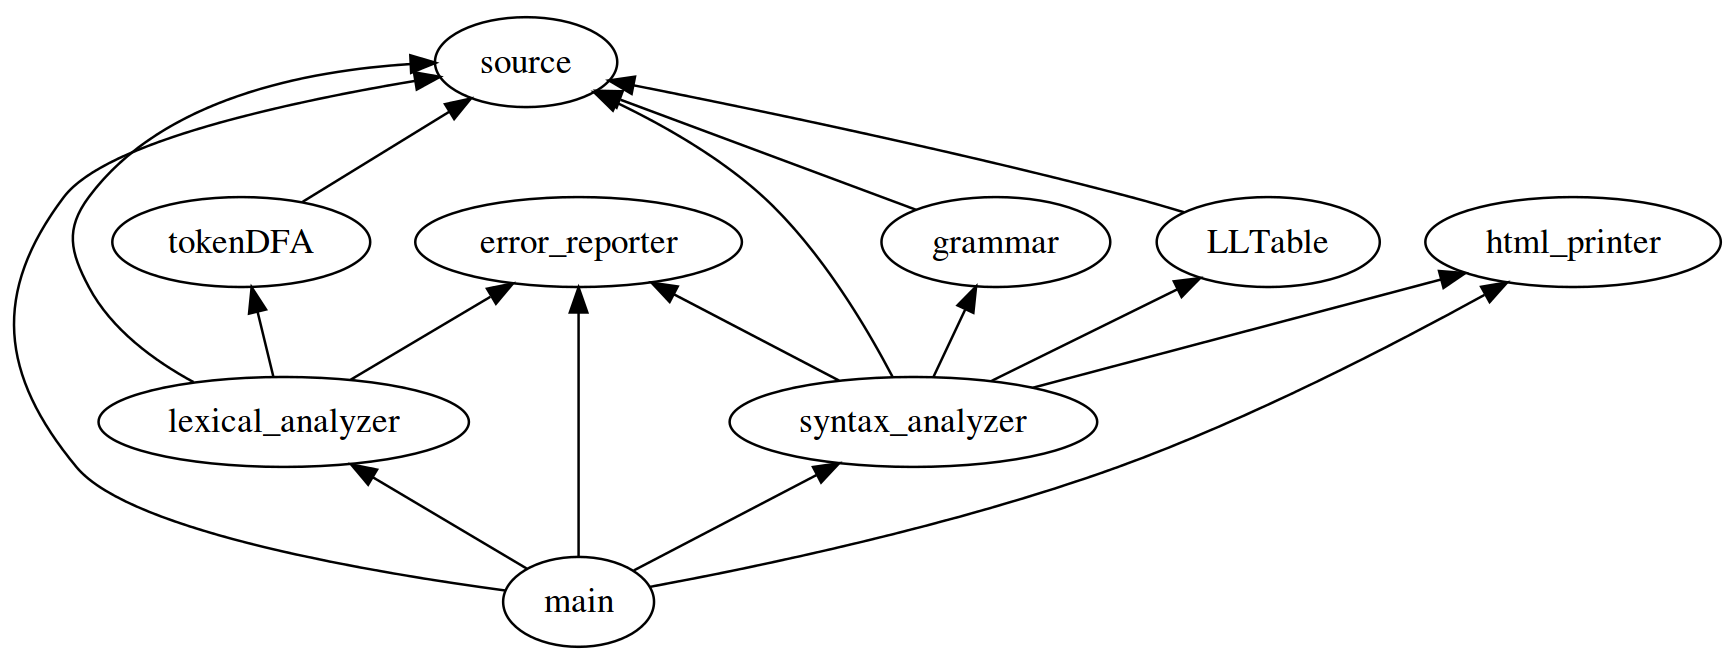
\includegraphics[width=\textwidth]{image/dependancy.png}
\captionof{figure}{函数依赖关系}
}\\

\section{}

\end{document}
